% =========================================================
% multilingual_llm_review.tex  –  ACM Computing Surveys style
% Author : Prakhar Srivastava, IIIT Allahabad
% =========================================================

\documentclass[acmsmall,screen,review]{acmart}

\setcopyright{none}
\settopmatter{printacmref=false}
\renewcommand\footnotetextcopyrightpermission[1]{}

\ccsdesc[500]{Computing methodologies~Natural language processing}
\ccsdesc[300]{Information systems~Digital libraries and archives}
\ccsdesc[300]{Computing methodologies~Machine learning}

\acmJournal{CSUR}

% ---- packages ----
\usepackage{booktabs}
\usepackage{tabularx}
\usepackage{array}
\usepackage{multirow}
\usepackage{graphicx}
\usepackage{subcaption}
\usepackage{xcolor}
\usepackage{tikz}
\usetikzlibrary{shapes.geometric, arrows.meta, positioning, fit, calc, backgrounds}

% =========================================================
% TITLE
% =========================================================

\title[Multilingual Reliability of LLMs in Scientific IR]
{Evaluating Multilingual Reliability of Large Language Models in
Scientific Literature Analysis: A Review and Empirical Study of
Cross-Lingual Evidence Retrieval}

\subtitle{Integrating Cross-Lingual Factuality, Hallucination, and
Benchmarking Perspectives with a Hindi--English Retrieval Case Study
on SciFact}

% =========================================================
% AUTHOR
% =========================================================

\author{Prakhar Srivastava}
\affiliation{%
  \institution{Department of Information Technology, IIIT Allahabad}
  \country{India}
}
\email{pns2026002@iiita.ac.in}
\renewcommand{\shortauthors}{Prakhar Srivastava}

% =========================================================
% ABSTRACT
% =========================================================

\begin{abstract}
Automated scientific literature analysis using large language models
(LLMs) has seen a surge of interest, yet nearly all published
evaluations share one blind spot: the assumption that English-language
performance is a reasonable proxy for performance in other languages.
This paper argues that this assumption is fragile, and it supports
that argument in two complementary ways.  First, we review and
synthesise evidence from cross-lingual factuality studies, multilingual
benchmarking research, and automated literature-review evaluations,
organising findings around four interacting dimensions---language and
data resources, evaluation methodology, generation and grounding
mechanisms, and application-level quality control.  The review shows
that multilingual capability is heterogeneous: benchmarks consistently
document performance gaps across language-resource levels, factual
knowledge can be encoded inconsistently across languages, and automated
review systems continue to hallucinate references even in well-resourced
settings.

Second, we present an original empirical study---\emph{Cross-Lingual
Scientific Evidence Retrieval: Measuring the Hindi--English Retrieval
Gap on SciFact}---that instantiates one piece of this broader problem in
a controlled, reproducible setting.  Using the BEIR SciFact benchmark
(5\,183 English biomedical abstracts, 300 test claims), we evaluated
three retrieval architectures---BM25, an English-only dense encoder
(\texttt{all-MiniLM-L6-v2}), and a multilingual dense encoder
(\texttt{paraphrase-multilingual-MiniLM-L12-v2})---under both English
and machine-translated Hindi queries across 1\,800 query-level
evaluations.  BM25 and the English encoder collapse under Hindi input
(Recall@5 drops from 0.70 and 0.74 to 0.09 and 0.03, respectively),
while multilingual dense retrieval narrows the gap to a Recall@5
difference of 0.35.  Nonetheless, 77\% of Hindi queries still fail to
retrieve any relevant abstract in the top ten, underscoring how far
current off-the-shelf tools fall short for cross-lingual scientific
evidence access.

Taken together, the review and the case study point to the same set of
unresolved problems: the absence of non-English scientific corpora,
the lack of a dedicated multilingual scientific-reliability benchmark,
and the persistent treatment of language as an afterthought in
retrieval and grounding pipelines.  The paper closes with concrete
directions for each of these gaps.
\end{abstract}

% =========================================================
% KEYWORDS
% =========================================================

\keywords{
  large language models,
  multilingual NLP,
  scientific evidence retrieval,
  cross-lingual consistency,
  hallucination,
  factuality,
  BM25,
  dense retrieval,
  SciFact,
  Hindi,
  low-resource languages
}

% =========================================================
\begin{document}
\maketitle
% =========================================================

% ---------------------------------------------------------
% SECTION 1 – INTRODUCTION
% ---------------------------------------------------------

\section{Introduction}
\label{sec:introduction}

Scientific publishing now produces millions of papers every year, spread
across dozens of languages and thousands of venues.  Keeping up with even
a narrow sub-field has become genuinely difficult for individual
researchers, which has driven growing interest in systems that can search,
screen, and synthesise literature automatically
\citep{scherbakov2025emergence,wu2025automated,tang2025automated}.  LLMs
are at the centre of that effort, and results in English have been
encouraging enough to push these tools into real research workflows.

What tends to get less attention is what happens when the user is not
writing in English.  Hindi speakers, for example, make up a substantial
share of the global scientific community, yet nearly every benchmark used
to evaluate scientific literature systems was designed around English
claims matched against English corpora.  The gap between what gets
measured and what actually matters in practice is easy to overlook until
something goes wrong.

The multilingual literature itself offers a warning.  Models such as mT5
and BLOOM were trained on data spanning dozens of languages
\citep{xue2021mt5,bigscience2022bloom}, and benchmarks like XTREME
confirmed that cross-lingual transfer is possible in principle
\citep{hu2020xtreme}.  But possibility is not uniformity.  MMLU-ProX,
which tests the same reasoning questions in 29 languages simultaneously,
found performance gaps between high-resource and low-resource languages
that are difficult to explain away as noise \citep{xuan2025mmlupro}.
Factuality research adds a sharper concern: a model can answer a question
correctly in English while producing a materially different response to an
equivalent question posed in another language
\citep{qi2023crosslingual,xue2024mlingconf}.

For scientific evidence retrieval---the step that must happen before any
LLM can reason over source material---these asymmetries translate directly
into unequal access to the scientific record.  If a retriever cannot
locate relevant abstracts when the query is in Hindi, whatever LLM sits
downstream is simply working without evidence.  That failure mode is both
practically important and, until recently, almost completely unstudied.

This paper addresses the problem in two ways.  The first part reviews and
synthesises the existing literature on multilingual reliability in
LLM-assisted scientific analysis, covering model and data conditions,
evaluation methodology, retrieval and grounding mechanisms, and quality
control at the application level.  The second part reports an original
empirical investigation that directly measures the Hindi--English retrieval
gap on the BEIR SciFact benchmark, using three retrieval architectures
under matched experimental conditions.  Connecting the review to a
concrete case study lets us ground the abstract conclusions in numbers
that can be reproduced and built upon.

Three questions organise the paper:
\begin{enumerate}
  \item What does available empirical work tell us about how multilingual
        reliability shifts across languages in scientific literature
        contexts?
  \item Which approaches have shown promise in narrowing these gaps, and
        where do they still fall short?
  \item What resources and evaluation designs does the field need to make
        meaningful progress?
\end{enumerate}

Section~\ref{sec:scope} defines the review scope.
Section~\ref{sec:background} covers multilingual models, benchmarks, and
prior literature-review automation work.
Section~\ref{sec:reliability} synthesises evidence on factuality,
hallucination, and resource asymmetry.
Section~\ref{sec:empirical} presents the empirical study in full, including
the system design, the pipeline flowchart, results tables, and error
analysis.
Section~\ref{sec:approaches} discusses mitigation strategies.
Section~\ref{sec:challenges} enumerates methodological challenges, and
Section~\ref{sec:gaps} identifies research gaps before the conclusion in
Section~\ref{sec:conclusion}.

% ---------------------------------------------------------
% SECTION 2 – SCOPE
% ---------------------------------------------------------

\section{Review Scope and Synthesis Framework}
\label{sec:scope}

This is a structured narrative review rather than a statistical
meta-analysis.  The literature is grouped around the intersection of
multilingual LLM reliability and scientific literature analysis, drawing
on four evidence categories: multilingual model development, cross-lingual
evaluation and factuality, LLM-assisted literature-review automation, and
mitigation and quality-control approaches.

The synthesis emphasises measurable findings and recurring methodological
limitations.  Studies are not treated as directly comparable unless they
share a common evaluation setting; instead, convergent findings across
different settings are noted where they appear.

Figure~\ref{fig:taxonomy} presents the taxonomy underlying the review.
Reliability is decomposed into four interacting layers: language and data
conditions, evaluation design, generation and grounding mechanisms, and
application-level controls.  This decomposition matters because an
observed reliability difference could arise at any layer, and attributing
it to the wrong one leads to interventions that miss the actual problem.

% --- Conceptual framework figure ---
\begin{figure}[t]
\centering
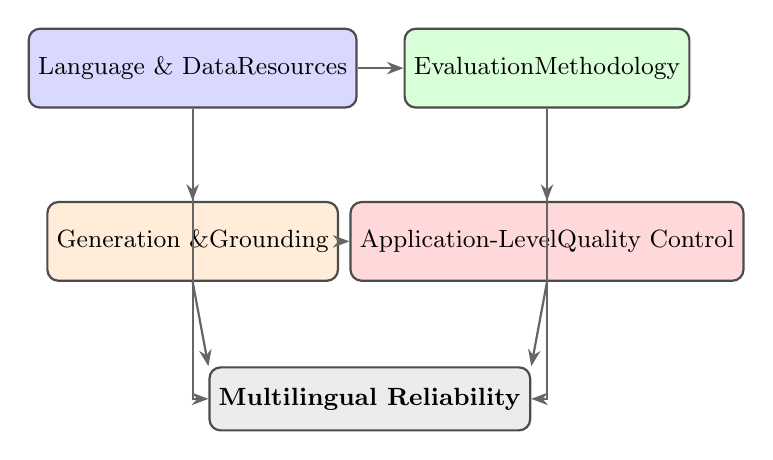
\begin{tikzpicture}[
  font=\small,
  box/.style={rectangle, rounded corners=4pt, draw=black!70, thick,
              text centered, minimum height=1cm, minimum width=3.6cm,
              fill=#1!15},
  arr/.style={-{Stealth[length=6pt]}, thick, draw=black!60}
]
  \node[box=blue]  (data)  at (0,0)    {Language \& Data\\Resources};
  \node[box=green] (eval)  at (4.5,0)  {Evaluation\\Methodology};
  \node[box=orange](gen)   at (0,-2.2) {Generation \&\\Grounding};
  \node[box=red]   (ctrl)  at (4.5,-2.2){Application-Level\\Quality Control};

  \node[box=gray, minimum width=2cm, minimum height=0.8cm]
        (rel) at (2.25,-4.2) {\textbf{Multilingual Reliability}};

  \draw[arr] (data) -- (eval);
  \draw[arr] (data) -- (gen);
  \draw[arr] (eval) -- (ctrl);
  \draw[arr] (gen)  -- (ctrl);
  \draw[arr] (data.south) |- (rel.west);
  \draw[arr] (eval.south) |- (rel.east);
  \draw[arr] (gen.south)  -- (rel.north west);
  \draw[arr] (ctrl.south) -- (rel.north east);
\end{tikzpicture}
\caption{Conceptual framework used in this review.  Multilingual
reliability in LLM-based scientific literature analysis is treated as an
outcome shaped by four interacting layers.  An observed reliability gap
may originate at any layer, so stage-specific evaluation is preferable to
a single aggregate score.}
\Description{Directed diagram showing four boxes---Language \& Data
Resources, Evaluation Methodology, Generation \& Grounding, Application
Quality Control---feeding into Multilingual Reliability.}
\label{fig:taxonomy}
\end{figure}

% ---------------------------------------------------------
% SECTION 3 – BACKGROUND
% ---------------------------------------------------------

\section{Background and Related Work}
\label{sec:background}

\subsection{Multilingual Large Language Models}
\label{sec:multilingual-models}

Work on multilingual language modelling accelerated substantially when
sequence-to-sequence pretraining was adapted to cover many languages at
once.  mT5 extended the T5 architecture to 101 languages by training on a
Common Crawl subset that was filtered to balance language representation
\citep{xue2021mt5}.  BLOOM subsequently demonstrated that a 176-billion
parameter model could be trained openly on a deliberately curated
multilingual corpus spanning 46 natural languages
\citep{bigscience2022bloom}.  GPT-4 reports multilingual benchmark numbers
but provides limited detail on how performance varies across languages or
scientific domains \citep{openai2023gpt4}.

What these models share is that their training corpora differ enormously
in size across languages.  English typically dominates by an order of
magnitude or more.  The implication is that multilingual capability as
measured by benchmark averages can obscure wide within-model variation:
the same model that performs well on Spanish may behave differently on
Hindi, and both may fall short on specialised scientific text.  XTREME
made this explicit by evaluating 40 languages across 9 tasks and finding
substantial spread even within individual tasks \citep{hu2020xtreme}.

\subsection{LLMs for Scientific Literature Analysis}
\label{sec:lit-review-automation}

There is a growing body of work examining how LLMs behave at each stage
of a literature-review workflow.  Scherbakov et al.\ conducted a
systematic review of LLM applications in this area and found that
GPT-based systems dominate the published literature, with performance
varying noticeably across workflow stages \citep{scherbakov2025emergence}.
Wu et al.\ built an end-to-end automated review-generation system that
incorporates layered quality-control checks at multiple pipeline stages
\citep{wu2025automated}.  Tang et al.\ evaluated three specific subtasks
---reference generation, abstract writing, and full review composition---
and found that even the strongest models produce hallucinated references at
a non-trivial rate, and that performance depends heavily on the
discipline \citep{tang2025automated}.

The limitation these studies share is their focus on English.  It is
reasonable to start there---most source literature is in English, and
annotation resources are richest in that language---but it creates a
situation where multilingual reliability is assumed rather than verified.

\subsection{Cross-Lingual Factuality and Confidence}
\label{sec:factuality-background}

Two research threads bear directly on the claims made in this paper.  The
first is cross-lingual factual consistency.  Qi et al.\ introduced
Ranking-based Consistency (RankC) to measure whether a model encodes the
same factual content when queried in different languages
\citep{qi2023crosslingual}.  Their finding that model scale does not
reliably improve cross-lingual consistency is worth emphasising: a larger
model can be simultaneously more accurate in English and less consistent
across languages.

The second thread concerns confidence calibration.  Xue et al.'s
MlingConf study showed that LLMs exhibit language-dominance effects in
their confidence outputs, and that prompting in the query-relevant
language can partly correct this behaviour for language-specific tasks
\citep{xue2024mlingconf}.  For scientific use, miscalibrated confidence
is particularly dangerous because a user who treats high model confidence
as a validity signal can propagate an error through an entire review.

% ---------------------------------------------------------
% SECTION 4 – RELIABILITY
% ---------------------------------------------------------

\section{Multilingual Reliability in Scientific Literature Analysis}
\label{sec:reliability}

\subsection{Cross-Lingual Performance and Resource Asymmetry}
\label{sec:resource-asymmetry}

The benchmarks reviewed here converge on a common finding: multilingual
performance is uneven, and the unevenness correlates with how much
training data a language has.  XTREME showed this across 40 languages and
9 tasks \citep{hu2020xtreme}; MMLU-ProX replicated it on reasoning tasks
across 29 languages, with the gap between high-resource and low-resource
languages remaining substantial \citep{xuan2025mmlupro}.

For scientific applications, this matters for a reason that general
benchmarks do not capture: scientific terminology tends to be
underrepresented in non-English training corpora independently of the
language's overall resource level.  A model that can handle conversational
Hindi may still stumble on biomedical Hindi, because biomedical Hindi
appears infrequently in web text.  Language-resource and domain-resource
constraints therefore pile on top of each other, and they are not easy to
separate without purpose-built evaluation data.

\subsection{Factual Consistency Across Languages}
\label{sec:factual-consistency}

Cross-lingual factual inconsistency has an obvious connection to
scientific use: if a model answers a question correctly in English but
differently in Hindi, then Hindi-speaking researchers are receiving
unequal access to the same scientific knowledge, mediated by the same
system.  Qi et al.'s RankC analysis provides concrete evidence that this
kind of inconsistency occurs and that it cannot be fixed simply by scaling
the model \citep{qi2023crosslingual}.

For literature synthesis, the problem appears at multiple stages.  A
retrieval failure in the query language means the downstream model never
sees the relevant evidence.  An extraction error in a non-English
document means the extracted information may differ from what a native
reader would extract.  Evaluating only the final answer, as most current
systems do, hides where these failures originate.

\subsection{Hallucination and Citation Reliability}
\label{sec:hallucination}

Hallucination---the generation of plausible-sounding but factually
unsupported text---is the failure mode that attracts most attention in
LLM-assisted literature analysis, and for good reason.  Tang et al.'s
evaluation found hallucinated references even in outputs from the
strongest models tested \citep{tang2025automated}.  Wu et al.'s layered
verification approach reduces this problem but does not eliminate it
entirely \citep{wu2025automated}.

The multilingual setting compounds the challenge.  Verification typically
works by checking generated claims against indexed source material.  Where
the source index has weak coverage for a language---fewer abstracts, less
metadata, narrower keyword matching---the verification step is working
against a smaller and potentially unrepresentative sample.  Quality
control inherits whatever asymmetry exists in the retrieval layer beneath
it.

\subsection{Domain-Specific Gaps}
\label{sec:domain-gaps}

General-purpose multilingual benchmarks do not test the specific
challenges of scientific text: specialised terminology, numerical claims,
methodological descriptions, citation networks, and claim-evidence
pairing.  A model can score well on MMLU-ProX in a given language while
still failing on domain-specific tasks in that language.  The gap between
general language capability and scientific reliability is therefore a
distinct research target, not simply a corollary of the general
multilingual gap.

\subsection{Confidence and Downstream Risk}
\label{sec:confidence-risk}

Confidence scores matter in scientific workflows because they influence
whether a user accepts or questions a model output.  MlingConf documents
that these scores can behave differently across languages and that the
direction of miscalibration is not uniform \citep{xue2024mlingconf}.  In
practice, a user who does not know that confidence is poorly calibrated
for their query language has no way of adjusting their scepticism
appropriately.

% ---------------------------------------------------------
% SECTION 5 – EMPIRICAL STUDY
% ---------------------------------------------------------

\section{Empirical Case Study: Hindi--English Retrieval Gap on SciFact}
\label{sec:empirical}

The review in the preceding sections establishes that cross-lingual
reliability problems are real and consequential.  What it cannot do, on
its own, is quantify how large those problems are in a specific
retrieval setting.  This section addresses that gap with an original
experiment that measures the Hindi--English retrieval gap on the BEIR
SciFact benchmark under three retrieval architectures.

\subsection{Pipeline Architecture}
\label{sec:pipeline}

Figure~\ref{fig:pipeline} shows the full system pipeline.  The key
components and the external resources used at each step are described
below.

% --- Pipeline Flowchart ---
\begin{figure*}[t]
\centering
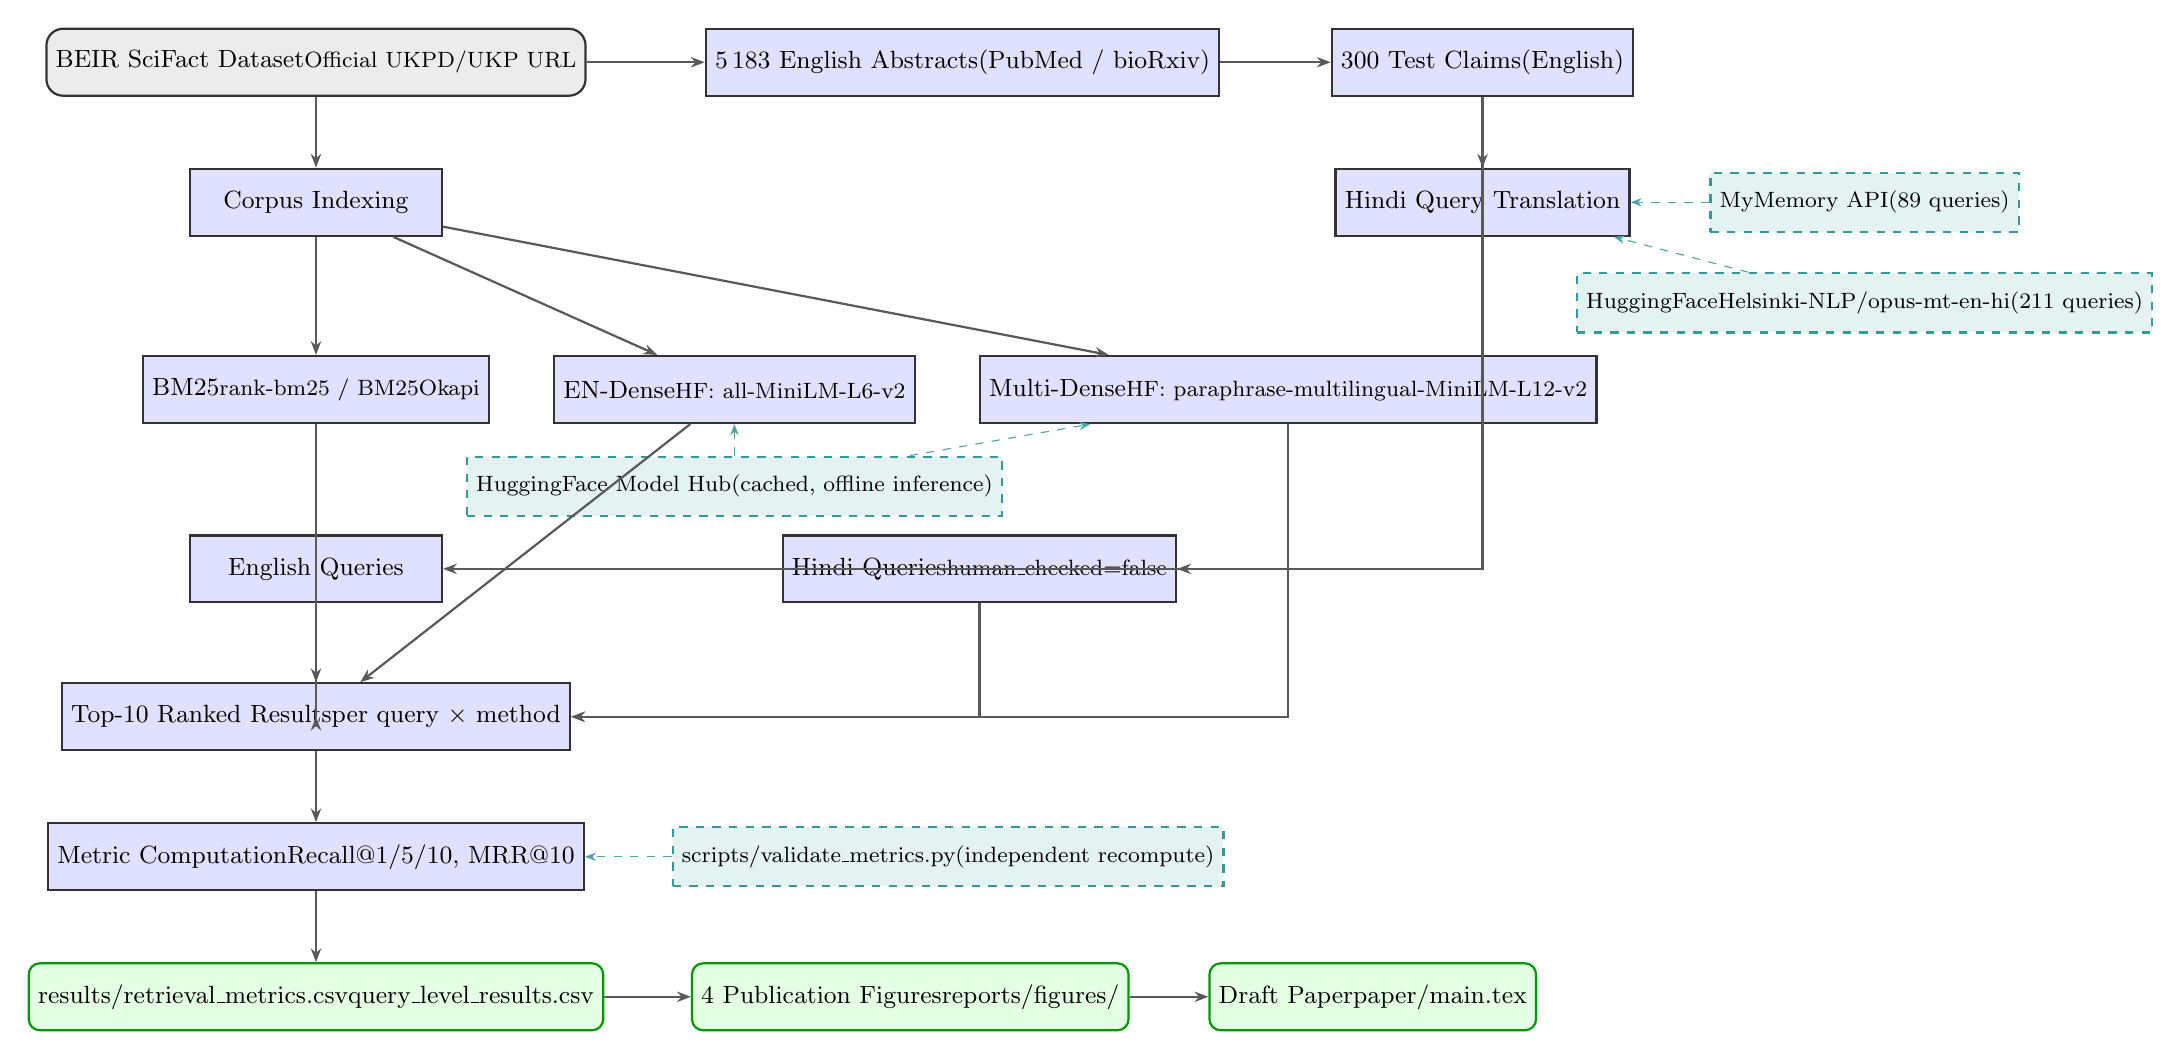
\begin{tikzpicture}[
  font=\small,
  node distance = 0.6cm and 1.1cm,
  startstop/.style={rectangle, rounded corners=6pt, draw=black!80,
                    thick, fill=gray!15, text centered,
                    minimum height=0.85cm, minimum width=3.2cm},
  process/.style={rectangle, draw=black!80, thick,
                  fill=blue!12, text centered,
                  minimum height=0.85cm, minimum width=3.2cm},
  decision/.style={diamond, aspect=2.4, draw=black!80, thick,
                   fill=orange!18, text centered,
                   minimum height=0.85cm, inner sep=1pt},
  api/.style={rectangle, draw=teal!80, thick, fill=teal!10,
              dashed, text centered,
              minimum height=0.75cm, minimum width=2.8cm, font=\footnotesize},
  result/.style={rectangle, rounded corners=4pt, draw=green!60!black,
                 thick, fill=green!10, text centered,
                 minimum height=0.85cm, minimum width=3.2cm},
  arr/.style={-{Stealth[length=5pt]}, thick, draw=black!65},
  apiline/.style={-{Stealth[length=4pt]}, dashed, draw=teal!70},
]

% Row 1 – data sources
\node[startstop] (beir)  {BEIR SciFact Dataset\\{\footnotesize Official UKPD/UKP URL}};
\node[process,   right=1.5cm of beir] (corpus) {5\,183 English Abstracts\\(PubMed / bioRxiv)};
\node[process,   right=1.4cm of corpus](queries){300 Test Claims\\(English)};

% Row 2 – translation
\node[process, below=0.9cm of queries] (translate) {Hindi Query Translation};
\node[api, right=1.0cm of translate]   (mymem)     {MyMemory API\\(89 queries)};
\node[api, below=0.5cm of mymem]       (opus)      {HuggingFace\\Helsinki-NLP/opus-mt-en-hi\\(211 queries)};

% Row 3 – retrieval branch
\node[process, below=0.9cm of beir]   (index)  {Corpus Indexing};

% Row 4 – three retrieval arms (side by side)
\node[process, below=1.5cm of index]  (bm25)  {BM25\\{\footnotesize rank-bm25 / BM25Okapi}};
\node[process, right=0.8cm of bm25]   (endense){EN-Dense\\{\footnotesize HF: all-MiniLM-L6-v2}};
\node[process, right=0.8cm of endense](mdense) {Multi-Dense\\{\footnotesize HF: paraphrase-multilingual-\\MiniLM-L12-v2}};

% HuggingFace note
\node[api, below=0.4cm of endense]    (hfhub) {HuggingFace Model Hub\\(cached, offline inference)};

% Row 5 – query fan-in
\node[process, below=1.4cm of bm25]   (enq)   {English Queries};
\node[process, right=4.3cm of enq]    (hiq)   {Hindi Queries\\{\footnotesize human\_checked=false}};

% Row 6 – ranked results
\node[process, below=1.0cm of enq]    (rank)  {Top-10 Ranked Results\\per query $\times$ method};

% Row 7 – evaluation
\node[process, below=0.9cm of rank]   (eval)  {Metric Computation\\Recall@1/5/10, MRR@10};
\node[api, right=1.1cm of eval]       (vscript){scripts/validate\_metrics.py\\(independent recompute)};

% Row 8 – outputs
\node[result, below=0.9cm of eval]    (csv)   {results/retrieval\_metrics.csv\\query\_level\_results.csv};
\node[result, right=1.1cm of csv]     (figs)  {4 Publication Figures\\reports/figures/};
\node[result, right=1.0cm of figs]    (paper) {Draft Paper\\paper/main.tex};

% ---- arrows ----
\draw[arr] (beir)    -- (corpus);
\draw[arr] (beir)    -- (index);
\draw[arr] (corpus)  -- (queries);
\draw[arr] (queries) -- (translate);
\draw[arr] (index)   -- (bm25);
\draw[arr] (index)   -- (endense);
\draw[arr] (index)   -- (mdense);

\draw[apiline] (mymem) -- (translate);
\draw[apiline] (opus)  -- (translate);
\draw[apiline] (hfhub) -- (endense);
\draw[apiline] (hfhub) -- (mdense);

\draw[arr] (enq)      -- (rank);
\draw[arr] (hiq)      |- (rank);
\draw[arr] (translate) |- (hiq);
\draw[arr] (queries)   |- (enq);

% retrieval arms → ranked results
\draw[arr] (bm25)    |- (rank);
\draw[arr] (endense) -- (rank);
\draw[arr] (mdense)  |- (rank);

\draw[arr] (rank)  -- (eval);
\draw[apiline] (vscript) -- (eval);
\draw[arr] (eval)  -- (csv);
\draw[arr] (csv)   -- (figs);
\draw[arr] (figs)  -- (paper);

\end{tikzpicture}
\caption{End-to-end system pipeline for the cross-lingual evidence
retrieval case study.  Solid arrows show data flow; dashed teal arrows
indicate external tools or APIs used at each stage.  All HuggingFace
model weights are cached locally; no live API calls are made during
retrieval.  Hindi translations are explicitly flagged
\texttt{human\_checked=false} throughout the pipeline.}
\Description{Flowchart showing BEIR SciFact data flowing through corpus
indexing, Hindi translation (MyMemory API and HuggingFace OPUS-MT), three
retrieval arms (BM25, EN-Dense, Multi-Dense), metric evaluation, and
output CSV files and figures.}
\label{fig:pipeline}
\end{figure*}

\subsection{Dataset and Experimental Protocol}
\label{sec:data-protocol}

We used the official BEIR release of SciFact
\citep{thakur2021beir,wadden2020scifact}: 5\,183 biomedical abstracts as
the retrieval corpus, 300 expert-authored test claims as queries, and 339
query-document relevance judgements.  All document identifiers were
verified as unique; all 300 query identifiers appear in the relevance
judgements.  The dataset licence (CC-BY 4.0) permits this kind of
research use.

The experimental protocol---top-$k$ values $\{1, 5, 10\}$, primary
metric Recall@5, seed 42---was frozen in
\texttt{configs/experiment.yaml} before any comparative results were
examined.

\paragraph{Hindi translation.}
The 300 English claims were machine-translated to Hindi using two
complementary methods.  The MyMemory API handled 89 queries before
rate-limiting made it impractical.  The remaining 211 were translated
offline using the \texttt{Helsinki-NLP/opus-mt-en-hi} MarianMT model
loaded from the HuggingFace Hub with \texttt{local\_files\_only=True}.
Every translated row in \texttt{data/hindi\_queries.csv} records the
source text, translated text, translation method, and an explicit flag
\texttt{human\_checked=false}.  These translations are a stress test, not
human-authored scientific prose; we return to this limitation in
Section~\ref{sec:threats}.

\paragraph{Retrieval systems.}
Three systems were compared:
\begin{enumerate}
  \item \textbf{BM25}: \texttt{rank-bm25} (BM25Okapi), lowercase
        whitespace and punctuation tokenisation.
  \item \textbf{EN-Dense}: \texttt{sentence-transformers/all-MiniLM-L6-v2}
        (22.7M parameters, 384 dimensions), trained primarily on English
        web text; loaded via the HuggingFace Hub.
  \item \textbf{Multi-Dense}:
        \texttt{sentence-transformers/paraphrase-multilingual-MiniLM-L12-v2}
        (118M parameters, 384 dimensions), aligned across 50+ languages
        via multilingual knowledge distillation
        \citep{reimers2020multilingual}; loaded via the HuggingFace Hub.
\end{enumerate}
Dense corpus embeddings were cached to disk
(\texttt{data/beir/corpus\_emb\_*.npy}) to avoid repeated six-minute
CPU encoding passes.

\paragraph{Validation.}
Aggregate metrics were independently recomputed from
\texttt{results/query\_level\_results.csv} using
\texttt{scripts/validate\_metrics.py}.  Agreement between saved and
recomputed values was exact to within $10^{-9}$ across all 24 metric
cells.  Thirty-seven unit tests in \texttt{tests/test\_retrieval\_utils.py}
all passed (1.56 s on Python 3.14.2).

\subsection{Quantitative Results}
\label{sec:results-quant}

Table~\ref{tab:metrics} and Table~\ref{tab:gap} show the main results.
All numbers are taken directly from
\texttt{results/retrieval\_metrics.csv}.

\begin{table}[t]
\centering
\small
\caption{Aggregate retrieval metrics on BEIR SciFact (test split,
$N = 300$ queries).  Best Hindi value and best English value shown in
bold for each metric.  Multi-Dense = \texttt{paraphrase-multilingual-MiniLM-L12-v2};
EN-Dense = \texttt{all-MiniLM-L6-v2}.}
\label{tab:metrics}
\begin{tabular}{llcccc}
\toprule
Lang & System & R@1 & R@5 & R@10 & MRR@10 \\
\midrule
EN & BM25         & 0.492 & 0.697 & 0.754 & 0.594 \\
EN & EN-Dense     & 0.482 & \textbf{0.738} & \textbf{0.783} & \textbf{0.605} \\
EN & Multi-Dense  & 0.367 & 0.530 & 0.616 & 0.455 \\
\midrule
HI & BM25         & 0.062 & 0.085 & 0.095 & 0.074 \\
HI & EN-Dense     & 0.013 & 0.025 & 0.042 & 0.021 \\
HI & Multi-Dense  & \textbf{0.089} & \textbf{0.176} & \textbf{0.221} & \textbf{0.133} \\
\bottomrule
\end{tabular}
\end{table}

\begin{table}[t]
\centering
\small
\caption{Hindi--English performance gap
$\Delta = \text{Score}_{\text{EN}} - \text{Score}_{\text{HI}}$
(paired $t$-test, $n = 300$).  Smaller $\Delta$ is better.}
\label{tab:gap}
\begin{tabular}{lcccc}
\toprule
System & $\Delta$R@1 & $\Delta$R@5 & $\Delta$R@10 & $\Delta$MRR@10 \\
\midrule
BM25        & 0.430 & 0.612\,$\pm$\,0.054 & 0.659 & 0.520 \\
            & \multicolumn{4}{c}{\footnotesize$t=22.2$, $p<10^{-10}$} \\[2pt]
EN-Dense    & 0.469 & 0.713\,$\pm$\,0.051 & 0.742 & 0.584 \\
            & \multicolumn{4}{c}{\footnotesize$t=27.6$, $p<10^{-10}$} \\[2pt]
Multi-Dense & \textbf{0.278} & \textbf{0.354}\,$\pm$\,\textbf{0.056}
            & \textbf{0.395} & \textbf{0.322} \\
            & \multicolumn{4}{c}{\footnotesize$t=12.3$, $p<10^{-10}$} \\
\bottomrule
\end{tabular}
\end{table}

\subsection{Figures Generated from the Experiment}
\label{sec:result-figs}

Figures \ref{fig:fig1}--\ref{fig:fig4} were generated directly from
\texttt{results/retrieval\_metrics.csv} and
\texttt{results/query\_level\_results.csv} using
\texttt{scripts/plot\_results.py}.  None of the figures were manually
adjusted; they represent the unedited output of the pipeline.

\begin{figure}[t]
  \centering
  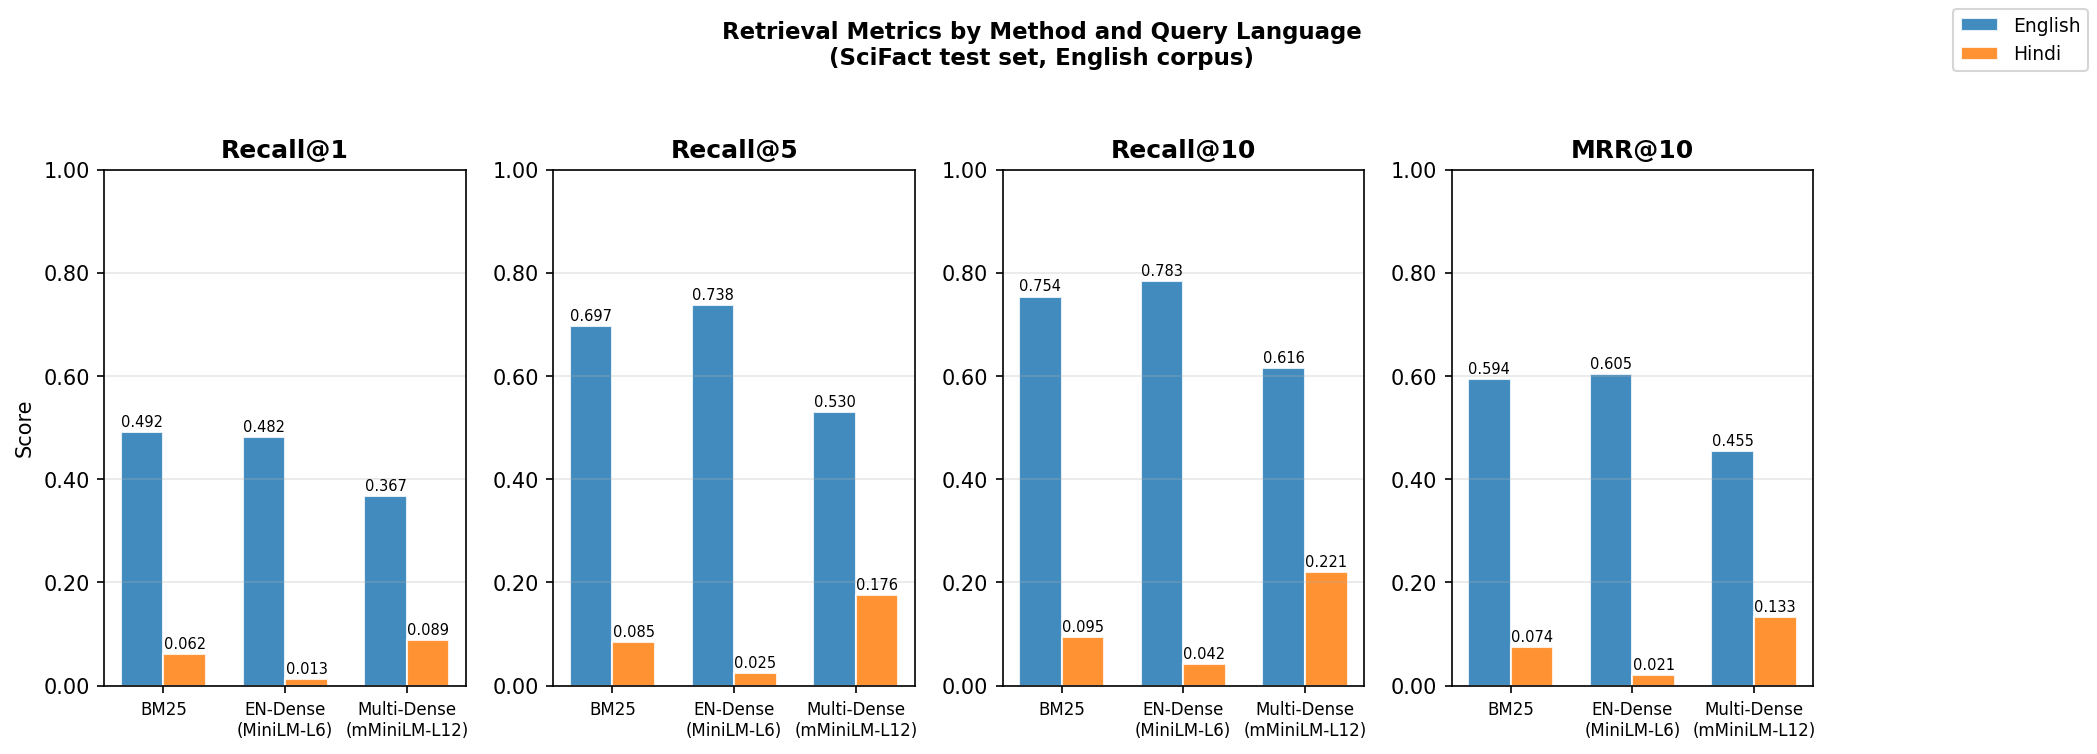
\includegraphics[width=\linewidth]{reports/figures/fig1_metric_comparison.png}
  \caption{Comparison of Recall@1, Recall@5, Recall@10, and MRR@10 across
  the three retrieval systems for English and Hindi queries.  The gap
  between the two language conditions is immediately apparent for all
  systems, but is smallest for Multi-Dense.}
  \Description{Bar chart comparing retrieval metrics for BM25, EN-Dense,
  and Multi-Dense under English and Hindi query conditions.}
  \label{fig:fig1}
\end{figure}

\begin{figure}[t]
  \centering
  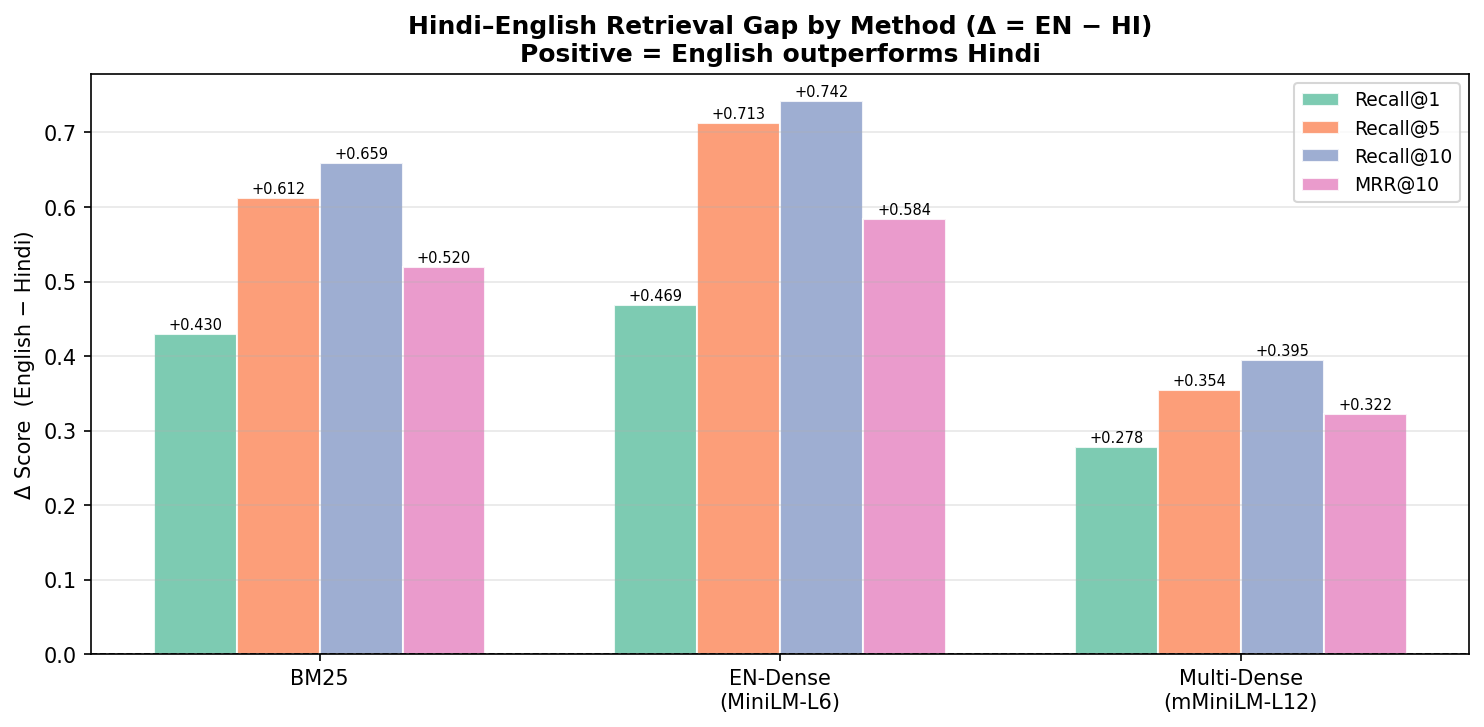
\includegraphics[width=\linewidth]{reports/figures/fig2_hindi_english_gap.png}
  \caption{Absolute Hindi--English performance gap ($\Delta$) for each
  retrieval system and metric.  Multi-Dense consistently shows the
  smallest gap, confirming that multilingual dense retrieval partially
  mitigates the cross-lingual deficit.}
  \Description{Bar chart showing the absolute difference in retrieval
  metrics between English and Hindi queries for three systems.}
  \label{fig:fig2}
\end{figure}

\begin{figure}[t]
  \centering
  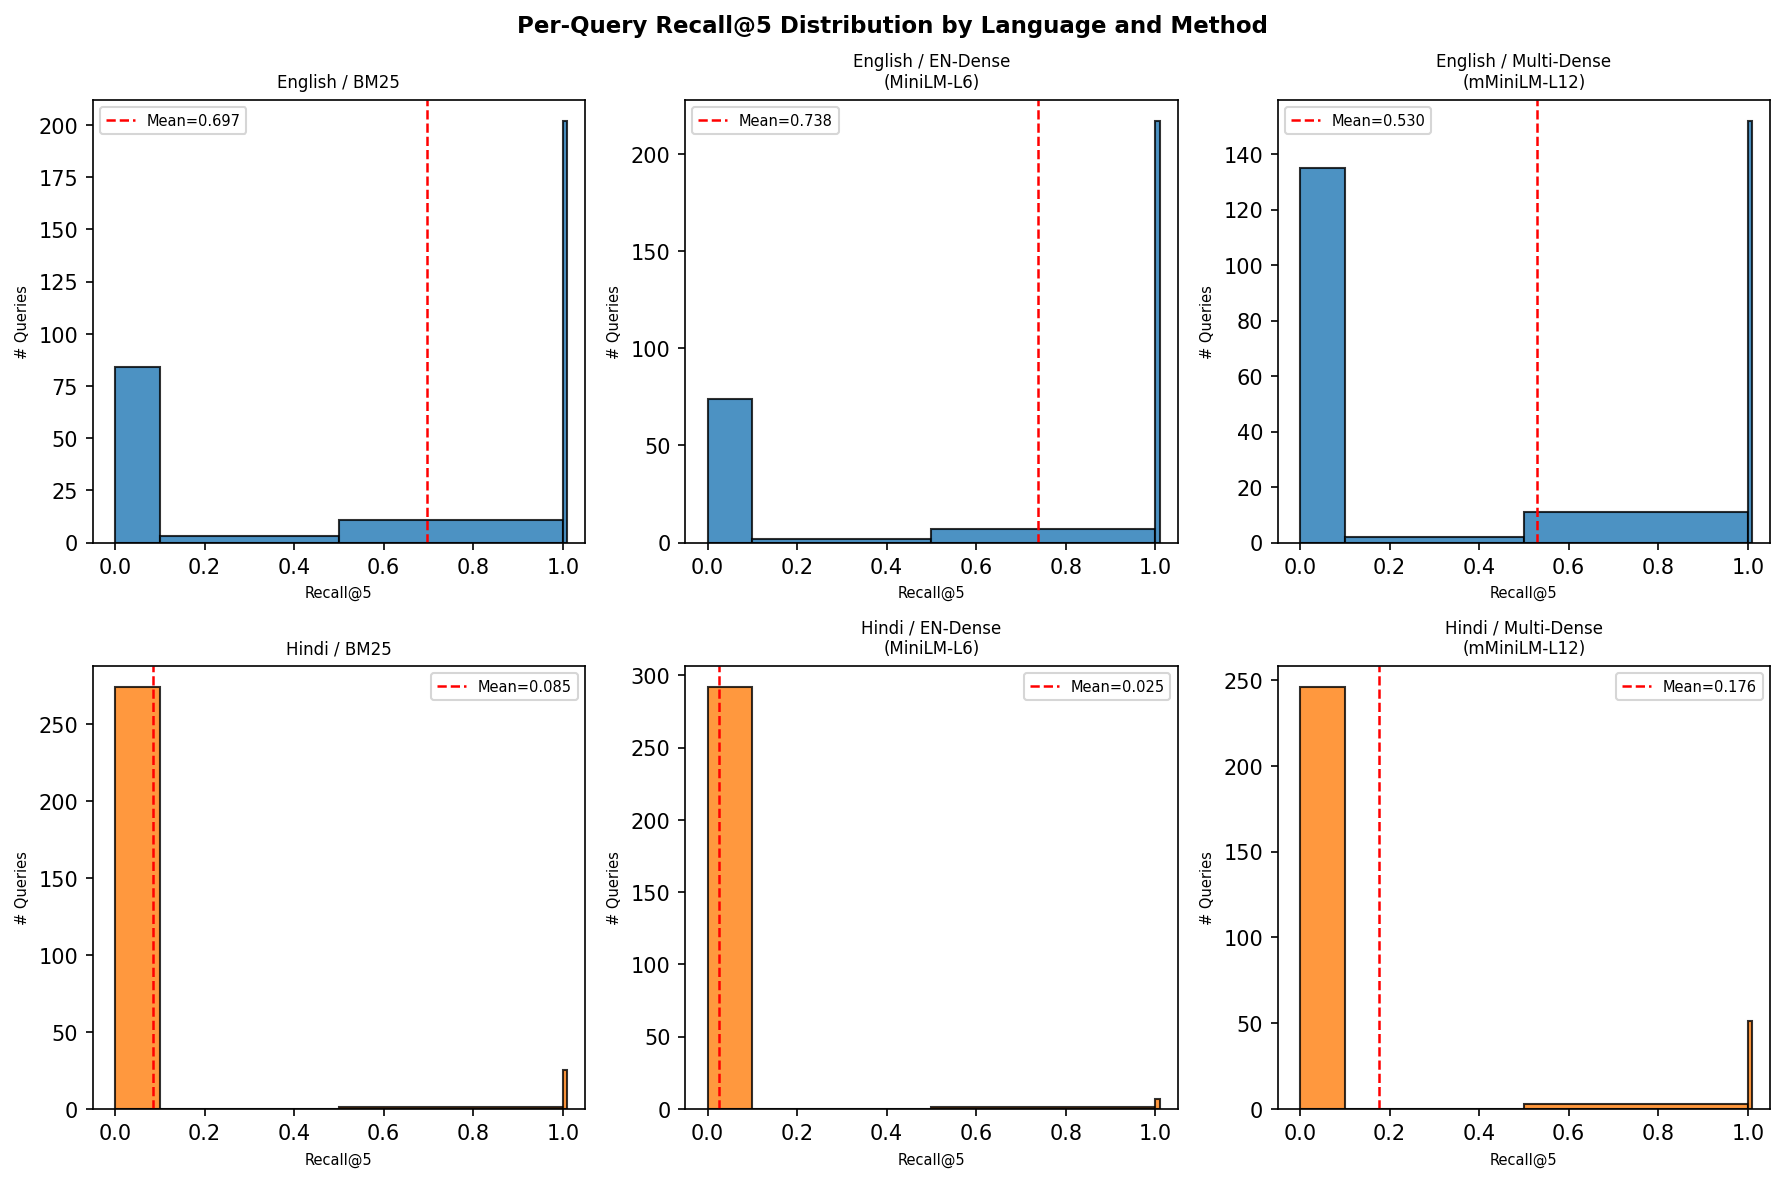
\includegraphics[width=\linewidth]{reports/figures/fig3_recall5_distributions.png}
  \caption{Per-query Recall@5 distributions for all six language$\times$system
  conditions.  Hindi distributions are dominated by zero values across all
  three systems, reflecting the high failure rate under translated queries.}
  \Description{Distribution plots of per-query Recall@5 showing high
  concentration at zero for Hindi queries.}
  \label{fig:fig3}
\end{figure}

\begin{figure}[t]
  \centering
  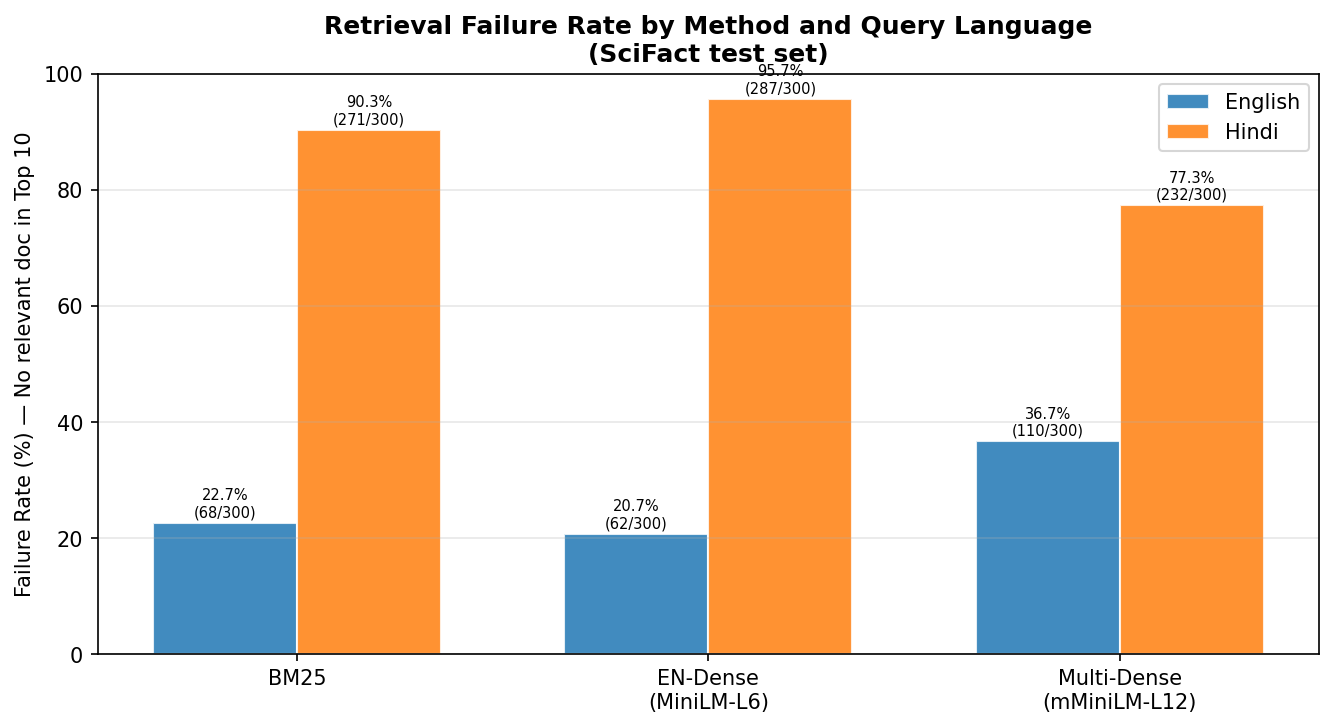
\includegraphics[width=\linewidth]{reports/figures/fig4_failure_rates.png}
  \caption{Proportion of queries with $\text{RR@10} = 0$ (complete failure
  to retrieve any relevant document in the top 10).  English failure rates
  range from 20--37\%; Hindi failure rates reach 77--96\%, with
  EN-Dense on Hindi recording the worst outcome (95.7\%).}
  \Description{Bar chart showing failure rates for each system and language,
  with Hindi failure rates substantially higher than English.}
  \label{fig:fig4}
\end{figure}

\subsection{Key Findings}
\label{sec:key-findings}

Three patterns in the results deserve emphasis.

\paragraph{Lexical retrieval partially survives, but only via untranslated tokens.}
BM25's Hindi Recall@5 (0.085) is non-trivial but vanishingly small
compared to its English result (0.697).  Inspection of the failure cases
shows that practically all non-zero BM25 hits on Hindi queries came from
claims that retained untranslated Latin abbreviations or numbers, such as
``PrP,'' ``1/2000,'' or ``UK.''  Queries composed entirely in Devanagari
scored zero reliably.

\paragraph{English dense retrieval is not a viable cross-lingual fallback.}
EN-Dense Recall@5 on Hindi is 0.025---roughly three percentage points
above chance.  This confirms that an encoder trained on English web text
cannot place Devanagari query vectors anywhere near the neighbourhood of
the relevant English abstract vectors.  The score is so low that routing
all queries through an English-only dense encoder would amount to
providing no retrieval at all for Hindi users.

\paragraph{Multilingual dense retrieval helps substantially, but not enough.}
Multi-Dense Recall@5 on Hindi (0.176) is seven times higher than
EN-Dense on Hindi (0.025) and statistically significantly better
($t = 6.93$, $p < 10^{-6}$).  The gap relative to English is also the
narrowest of the three systems ($\Delta = 0.354$ vs.\ $0.713$ for
EN-Dense).  However, 77.3\% of Hindi queries still return no relevant
result in the top 10, and Multi-Dense pays a 20-point Recall@5 penalty on
English queries relative to EN-Dense (0.530 vs.\ 0.738).  This trade-off
is familiar from the multilingual modelling literature and reflects
parameter sharing across 50+ languages in a 118M-parameter model
\citep{reimers2020multilingual,wang2020minilm}.

\subsection{Qualitative Error Analysis}
\label{sec:error-analysis}

Of the 1\,030 total retrieval failures ($\text{RR@10} = 0$), 160 queries
succeeded under EN-Dense (Recall@5$>$0) but failed completely under
Multi-Dense in Hindi.  Manual inspection of a sample of these cases
revealed five recurrent error patterns.

\paragraph{Polysemy in scientific terminology.}
Query~1---\emph{``0-dimensional biomaterials show inductive
properties''}---was translated as \emph{``0 - आयामी बायोमैटेरियल्स
आगमनात्मक गुण दिखाते हैं।''}  The word ``inductive'' in the biomaterials
context means capable of stimulating cell differentiation.  The
translator rendered it as \emph{āgamanātmak} (inductive reasoning in
formal logic), producing a vector that sits far from any biomedical
abstract in embedding space.

\paragraph{Wrong sense of ambiguous verbs.}
Query~75 contained the phrase ``a polymeric structure that compromises
two subunits''---a malapropism for ``comprises.''  Machine translation
rendered this as \emph{samjhautā kartī hai} (makes a political
concession), which is semantically correct for the English word
``compromises'' but entirely wrong for the biomedical content.

\paragraph{Technical entity mistranslation.}
Query~42 refers to ``homozygous alpha (+)- thalassemia trait subjects.''
The phrase ``trait subjects'' was translated as \emph{lakshan vishyon}
(school study topics), breaking any chance of lexical or semantic overlap
with clinical abstracts.

\paragraph{Embedding space fragmentation.}
In several queries where the Hindi translation was semantically accurate,
Multi-Dense still failed.  Close reading of the retrieved abstracts
suggests that biomedical named entities written in Devanagari script map
to regions of the embedding space that are distant from their Latin-script
counterparts, even though the model was designed for cross-lingual
alignment.

\paragraph{Capacity dilution on specialised domains.}
Multi-Dense's lower English performance (Recall@5 = 0.530 vs.\ 0.738 for
EN-Dense) reflects a known property of compact multilingual models: when
the same parameter budget is shared across many languages, the per-language
capacity in specialised domains decreases.  This shows up most clearly
in biomedical retrieval, where terminology density is high.

\subsection{Threats to Validity}
\label{sec:threats}

Three validity concerns apply to the empirical results.

The most significant is \emph{machine translation quality}.  None of the
300 Hindi translations were reviewed by a bilingual domain expert.  The
observed retrieval degradation is therefore a compound of genuine
cross-lingual retrieval difficulty and translation errors; the two
contributions cannot be separated in the current design.

The second concern is \emph{domain and corpus scope}.  SciFact is a
single-domain (biomedical), English-only-corpus benchmark.  Results here
may not generalise to other scientific disciplines or to corpora that
already include non-English documents.

The third is the \emph{retrieval-versus-factuality distinction}.
Recall@$k$ measures whether a relevant abstract appears in the top-$k$
candidates.  It says nothing about whether a downstream model would
correctly extract and reason over the evidence in that abstract, nor about
whether the final generated answer is factually correct.

% ---------------------------------------------------------
% SECTION 6 – APPROACHES
% ---------------------------------------------------------

\section{Current Approaches and Developments}
\label{sec:approaches}

Table~\ref{tab:comparative} summarises the representative work discussed
throughout the paper.  No single approach handles every layer of the
reliability problem; each addresses a specific source of failure.

\begin{table*}[t]
\centering
\small
\caption{Comparative synthesis of representative work on multilingual
reliability and LLM-assisted scientific literature analysis.}
\label{tab:comparative}
\begin{tabularx}{\textwidth}{@{}p{0.14\textwidth}
                               p{0.14\textwidth}
                               p{0.17\textwidth}
                               X
                               p{0.17\textwidth}@{}}
\toprule
\textbf{Study} & \textbf{Focus} & \textbf{Data / Setting} &
\textbf{Main contribution} & \textbf{Limitation for this review} \\
\midrule
Xue et al.\ \citep{xue2021mt5} &
Multilingual pretraining & 101 languages &
Large-scale multilingual text-to-text transfer &
General capability $\neq$ scientific reliability \\
BigScience \citep{bigscience2022bloom} &
Open multilingual LLM & 46 languages &
Open large-scale multilingual model &
Broad coverage $\neq$ uniform domain performance \\
Hu et al.\ \citep{hu2020xtreme} &
Cross-lingual benchmarking & 40 languages, 9 tasks &
Systematic cross-lingual task comparison &
Not specific to scientific literature \\
Qi et al.\ \citep{qi2023crosslingual} &
Factual consistency & Multilingual factual probing &
Factual knowledge can be inconsistent across languages &
Focuses on factual probing, not full pipelines \\
Xue et al.\ \citep{xue2024mlingconf} &
Confidence estimation & Multilingual confidence tasks &
Language-dominance effects in LLM confidence &
Confidence is only one reliability component \\
Scherbakov et al.\ \citep{scherbakov2025emergence} &
Literature-review automation & Systematic review &
Maps LLM use across review workflow stages &
Evidence base dominated by English \\
Wu et al.\ \citep{wu2025automated} &
Automated review generation & 343 articles, 35 topics &
Layered quality-control for automated reviews &
Multilingual generalisability not established \\
Tang et al.\ \citep{tang2025automated} &
Review-generation evaluation & Multi-task evaluation &
Measures hallucination, coverage, consistency &
Primarily English-language evaluation \\
Xuan et al.\ \citep{xuan2025mmlupro} &
Multilingual reasoning & 29 languages, parallel &
Direct cross-lingual comparison; documents gaps &
Not designed for scientific IR workflows \\
Thakur et al.\ \citep{thakur2021beir} &
Zero-shot IR benchmarking & 18 datasets incl.\ SciFact &
Standardised multilingual IR evaluation framework &
All test datasets are English-corpus \\
\midrule
\textbf{This work} &
Cross-lingual evidence retrieval &
BEIR SciFact, EN+HI queries &
Empirical gap measurement; 1\,800 evaluations;
error analysis & Single language pair; machine-translated queries \\
\bottomrule
\end{tabularx}
\end{table*}

\subsection{Retrieval-Augmented Generation}
\label{sec:rag}

RAG grounds generation in retrieved source documents, reducing dependence
on parametric memory.  For scientific use, it can make citation checking
explicit: a system can verify that the abstract it cites was actually
retrieved and matches the generated claim.  The empirical results in
Section~\ref{sec:empirical} illustrate the upstream risk: if retrieval
fails under non-English queries, RAG has nothing useful to supply to the
generator.

\subsection{Cross-Lingual Reasoning and Knowledge Transfer}
\label{sec:crosslingual-reasoning}

One pragmatic response to weak retrieval in a low-resource language is to
route the query through a high-resource language as an intermediate
reasoning step.  Translate to English, retrieve in English, and return a
result in the original language.  This approach inherits the limitations
of machine translation---some of the same error modes documented in
Section~\ref{sec:error-analysis} apply---but it at least gives the
retriever a chance to find relevant material.

\subsection{Multilingual and Domain-Specific Fine-Tuning}
\label{sec:finetuning}

Fine-tuning on domain-specific multilingual data is conceptually
straightforward, but high-quality biomedical text in Hindi is scarce
enough that it is not currently a practical remedy.  The multilingual
dense encoder used in our experiments
(\texttt{paraphrase-multilingual-MiniLM-L12-v2}) was not fine-tuned on
biomedical data, which likely contributes to some of the domain-specific
failures documented above.

\subsection{Multilayered Quality Control}
\label{sec:quality-control}

Wu et al.'s verification pipeline \citep{wu2025automated} and Tang et
al.'s evaluation framework \citep{tang2025automated} both point in the
same direction: fluency is not a reliable proxy for correctness, so
explicit checking of citations, evidence alignment, and factual claims is
necessary.  For multilingual systems, these checks need to be designed to
work on source material that may be in a different language from the query.

% ---------------------------------------------------------
% SECTION 7 – CHALLENGES
% ---------------------------------------------------------

\section{Research Challenges and Limitations}
\label{sec:challenges}

\subsection{Scarcity of Non-English Scientific Corpora}
\label{sec:corpora}

The empirical study is a useful data point but it also illustrates the
larger problem.  SciFact is English-only.  The Hindi queries are
translations of English claims.  The situation---a translated query against
a monolingual English corpus---is a stress test, not a realistic model of
how a Hindi-speaking researcher would actually engage with literature.
Building corpora of naturally authored scientific claims in non-English
languages, with matched evidence documents and relevance judgements, would
make it possible to test a scenario that is both more realistic and more
demanding.

\subsection{Translation Artifacts in Benchmarks}
\label{sec:translation}

MMLU-ProX \citep{xuan2025mmlupro} and the Hindi queries used in our
experiment both rely on translation to create non-English test items.
Translation improves scalability but introduces systematic biases.  The
error modes documented in Section~\ref{sec:error-analysis} are partly a
consequence of this design choice, and they are hard to separate from
genuine cross-lingual retrieval difficulty without naturally authored
alternatives.

\subsection{Language--Domain Confounding}
\label{sec:confounding}

The experiments in this paper cannot tell us whether the Hindi retrieval
failures arise primarily from language-resource asymmetry, from
biomedical domain scarcity in Hindi training data, or from both.  Isolating
these factors requires a matched experimental design: the same scientific
task evaluated in multiple languages while holding the domain constant,
then repeated across domains within the same language.

\subsection{No Standardised Scientific-Reliability Benchmark}
\label{sec:metrics}

XTREME and MMLU-ProX provide important multilingual evaluation
infrastructure, but neither covers claim verification, citation grounding,
numerical fidelity, or methodological summarisation.  A purpose-built
multilingual scientific benchmark that tests these properties across a
range of languages would change the character of evaluation in this area.

\subsection{English-Centric Evidence Base}
\label{sec:english-bias}

Almost all published evaluations of automated literature-review systems
used English source material and English evaluation.  The conclusions those
studies draw about reliability may apply primarily to English users, but
they are often presented as general findings about LLM capability in
scientific contexts.

% ---------------------------------------------------------
% SECTION 8 – GAPS AND FUTURE DIRECTIONS
% ---------------------------------------------------------

\section{Research Gaps and Future Directions}
\label{sec:gaps}

\subsection{Multilingual Scientific Benchmarks}
\label{sec:benchmark-gap}

A dedicated multilingual scientific benchmark should include at minimum:
claim verification, citation grounding, numerical-claim fidelity, and
methodological summarisation.  Parallel construction across languages
(as in MMLU-ProX) is a reasonable starting design, but benchmark items
should be reviewed by bilingual domain experts independent of any LLM
assistance.

\subsection{Naturally Authored Non-English Scientific Corpora}
\label{sec:corpus-gap}

Translated test queries are a workable starting point but not a long-term
solution.  Corpora of naturally authored scientific claims and abstracts in
languages such as Hindi, Arabic, Chinese, and Portuguese---with expert
relevance annotations---would enable the kind of ecologically valid
evaluation that the field currently lacks.

\subsection{Disentangling Language and Domain Effects}
\label{sec:disentangle-gap}

Future experiments should vary language and domain independently rather
than conflating them.  Concretely: take a fixed set of biomedical claims,
test retrieval in several languages, and repeat the experiment in a
different scientific domain while holding the languages constant.  This
factorial design would clarify how much of the observed performance gap is
attributable to each factor.

\subsection{Cross-Lingual Retrieval and Grounding}
\label{sec:verification-gap}

The empirical results suggest that the most valuable near-term
investment for cross-lingual scientific retrieval is a multilingual dense
encoder trained specifically on scientific and biomedical text.
Off-the-shelf multilingual encoders show some cross-lingual capability,
but their biomedical term representations are noticeably weaker than those
of domain-adapted English encoders.  Retrieval recall, citation
correctness, and evidence-span alignment should all be reported metrics for
any such system.

\subsection{Transparent Reporting of Language Coverage}
\label{sec:reporting-gap}

A simple change in norms would make a material difference: studies
evaluating LLM-assisted literature analysis should explicitly report the
languages represented in their source corpus, retrieval index, evaluation
set, and verification procedures.  Without this information, readers
cannot know whether a reported reliability finding applies to their own
use case.

\subsection{A Descriptive Gap Measure}
\label{sec:gap-measure}

For comparison across studies, the gap between high-resource and
low-resource language conditions can be written as

\begin{equation}
\Delta R = R_{\mathrm{high}} - R_{\mathrm{low}},
\label{eq:reliability-gap}
\end{equation}

where $R_{\mathrm{high}}$ and $R_{\mathrm{low}}$ are the values of some
reliability metric for the two conditions.  Equation~\ref{eq:reliability-gap}
is a descriptive measure, not a universal benchmark; the underlying metric
and the definition of ``high-resource'' must be stated explicitly for the
comparison to be meaningful.  In our experiment, $\Delta R$ for
Multi-Dense (Recall@5) is 0.354, compared to 0.713 for EN-Dense.

Table~\ref{tab:research-gaps} summarises the five main gaps and their
corresponding research directions.

\begin{table}[t]
\centering
\small
\caption{Research gaps identified and corresponding future directions.}
\label{tab:research-gaps}
\begin{tabularx}{\linewidth}{@{}p{0.33\linewidth}X@{}}
\toprule
\textbf{Gap} & \textbf{Direction} \\
\midrule
Sparse non-English scientific data &
Build naturally authored multilingual scientific corpora with expert
relevance annotations. \\
No scientific-reliability benchmark &
Develop multilingual benchmarks covering claim verification, citation
grounding, and numerical fidelity. \\
Language/domain confounding &
Use factorial designs that vary language and scientific domain
independently. \\
Weak cross-lingual retrieval &
Fine-tune dense encoders on multilingual biomedical text; evaluate
retrieval recall and evidence alignment separately. \\
Opaque language coverage reporting &
Require explicit reporting of corpus, retrieval index, and evaluation
set languages in published studies. \\
\bottomrule
\end{tabularx}
\end{table}

% ---------------------------------------------------------
% SECTION 9 – CONCLUSION
% ---------------------------------------------------------

\section{Conclusion}
\label{sec:conclusion}

Three threads run through this paper.  The first is the finding, now
replicated across several benchmarking studies, that multilingual LLM
performance is not uniform: gaps between high-resource and low-resource
languages are substantial and do not disappear with scale
\citep{hu2020xtreme,qi2023crosslingual,xuan2025mmlupro}.

The second is the finding, from automated literature-review research, that
even English-language systems hallucinate references and produce factual
errors at non-trivial rates \citep{tang2025automated,wu2025automated}.
Adding a cross-lingual retrieval layer to an already imperfect generation
pipeline is likely to compound these problems rather than cancel them out.

The third thread is the empirical result presented in
Section~\ref{sec:empirical}.  Across 1\,800 controlled query evaluations
on a standard scientific retrieval benchmark, Hindi queries caused dramatic
performance degradation in two of the three systems tested and left 77\%
of queries completely unanswered even in the best system.  Multilingual
dense retrieval offered meaningful improvement but exacted a substantial
cost on English performance---a trade-off that reflects the limits of
compact shared-parameter models rather than a problem specific to any
single implementation.

The practical implication is straightforward: systems that present
LLM-assisted scientific literature analysis as a broadly available
capability should acknowledge that the capability is severely degraded for
non-English users under current technology.  The research implication is
equally clear: the field needs purpose-built multilingual scientific
corpora, standardised multilingual evaluation benchmarks, and dense
encoders trained on domain-specific multilingual data before the promise
of automated literature analysis can be delivered equitably across
languages.

% =========================================================
% REFERENCES
% =========================================================

\bibliographystyle{ACM-Reference-Format}
\bibliography{references_full}

\end{document}
